
\section{Time Averaged Result}

% Time Averaged Pbar to Proton Ratio
In August 2016, the AMS-02 collaboration published the time-averaged antiproton to proton flux ratio as a function of the rigidity for up to 450 GV, using data collected during the first four years of the experiment’s operation (May 2011 to May 2015) \cite{AMS02AntiprotonPRL2016}. In Feb 2021, the AMS-02 collaboration published the flux ratio for up to 525 GV using the data accumulated during the first six and a half years of operation \cite{PhysicsReport2}. The AMS-02 experiment has been still in operation collecting continuously cosmic data. With more data, the antiproton to proton flux ratio can be updated with higher statistics and improved accuracy. This thesis has used data of the first ten years of operation up to May 2021. In figure \ref{timeaveragedratio}, the final antiproton to proton flux ratio of this analysis is shown. \par

%\begin{figure}[H]
%\centering
%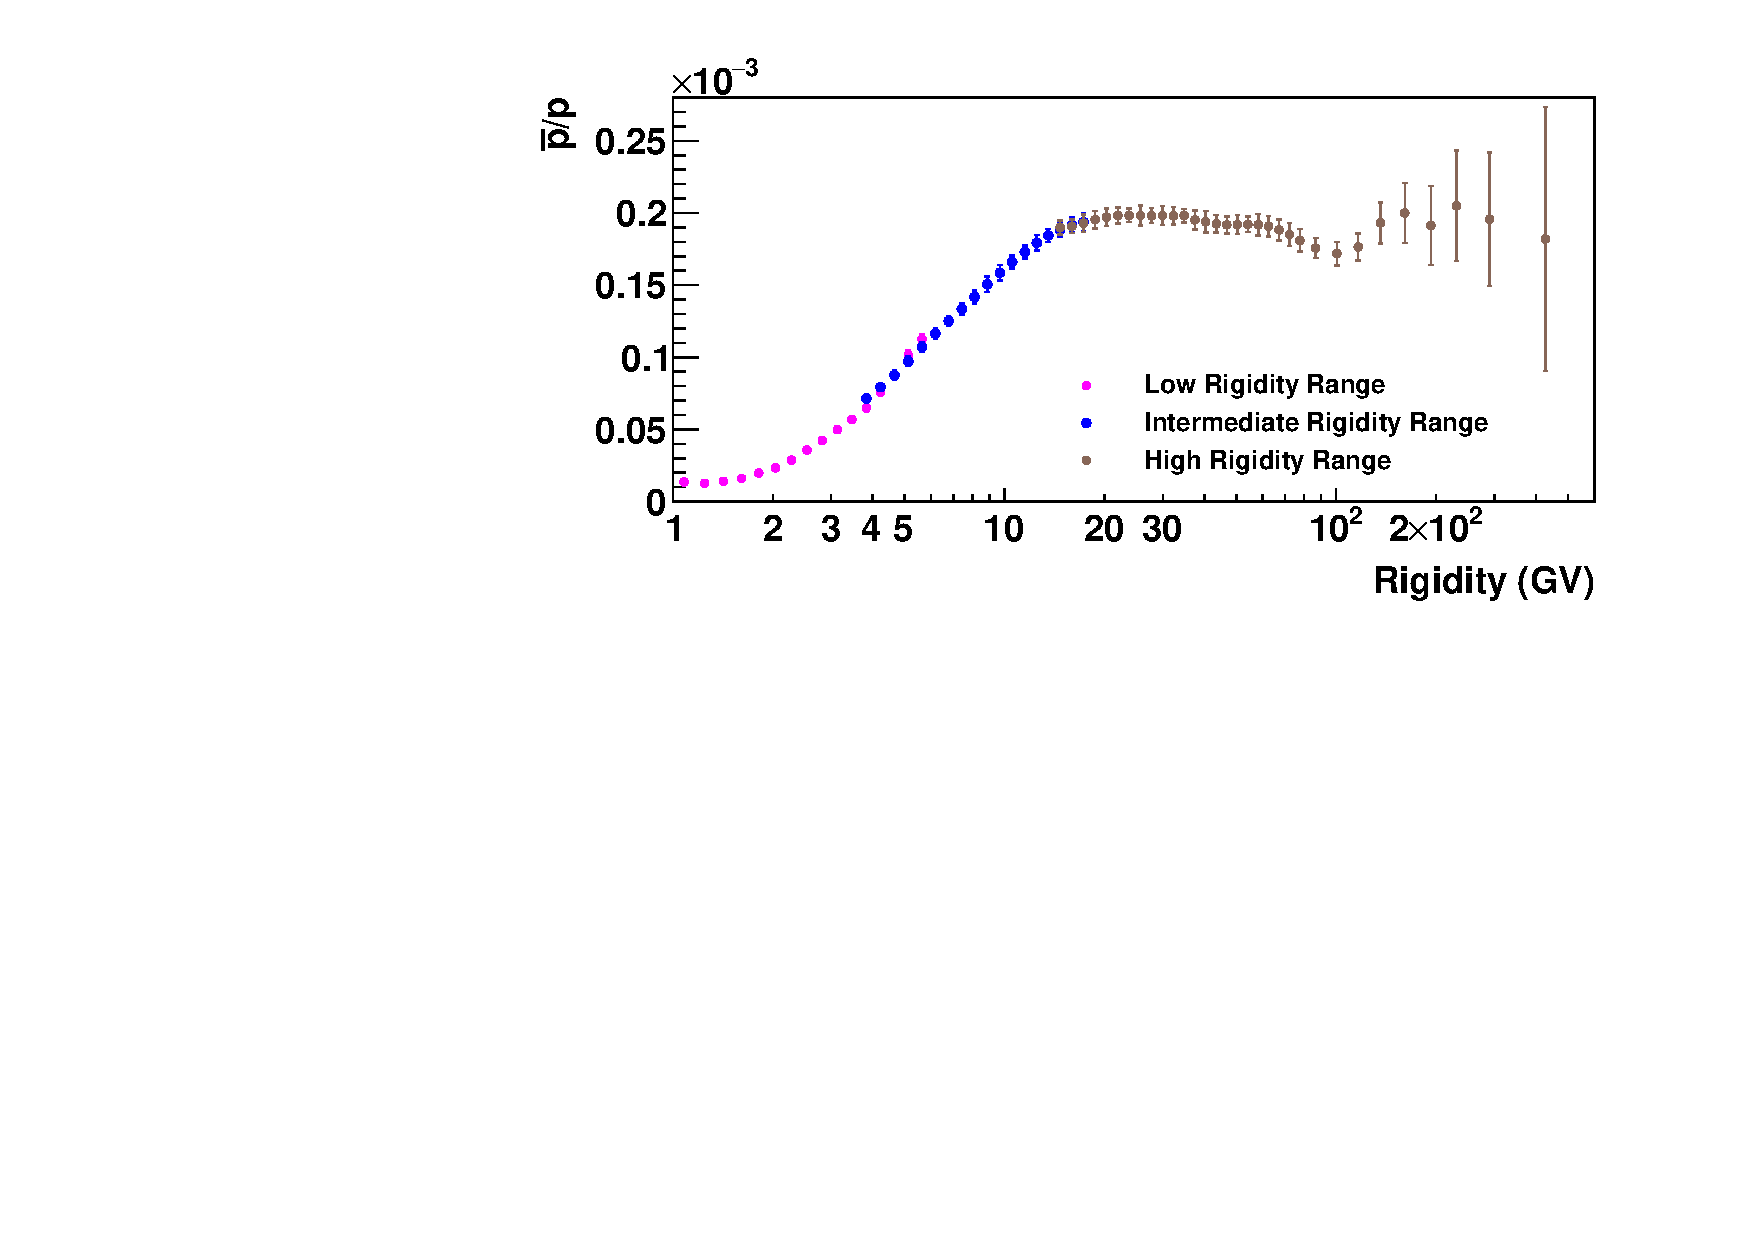
\includegraphics[width=1.00\textwidth, height=0.3\textheight]{Figures/chapter5/timeaveraged/fullratio_pass78.pdf}
%\caption{The time-averaged antiproton to proton flux ratio in three rigidity ranges. In the two overlapping ranges, the results from different template fit methods are consistent with each other. The error bars are the total errors calculated from the quadratic sum of the statistical and the systematic errors.}
%\label{timeaveragedratioWithOverlapping}
%\end{figure}

\begin{figure}[p]
    \centering
    \subfigure[]{
        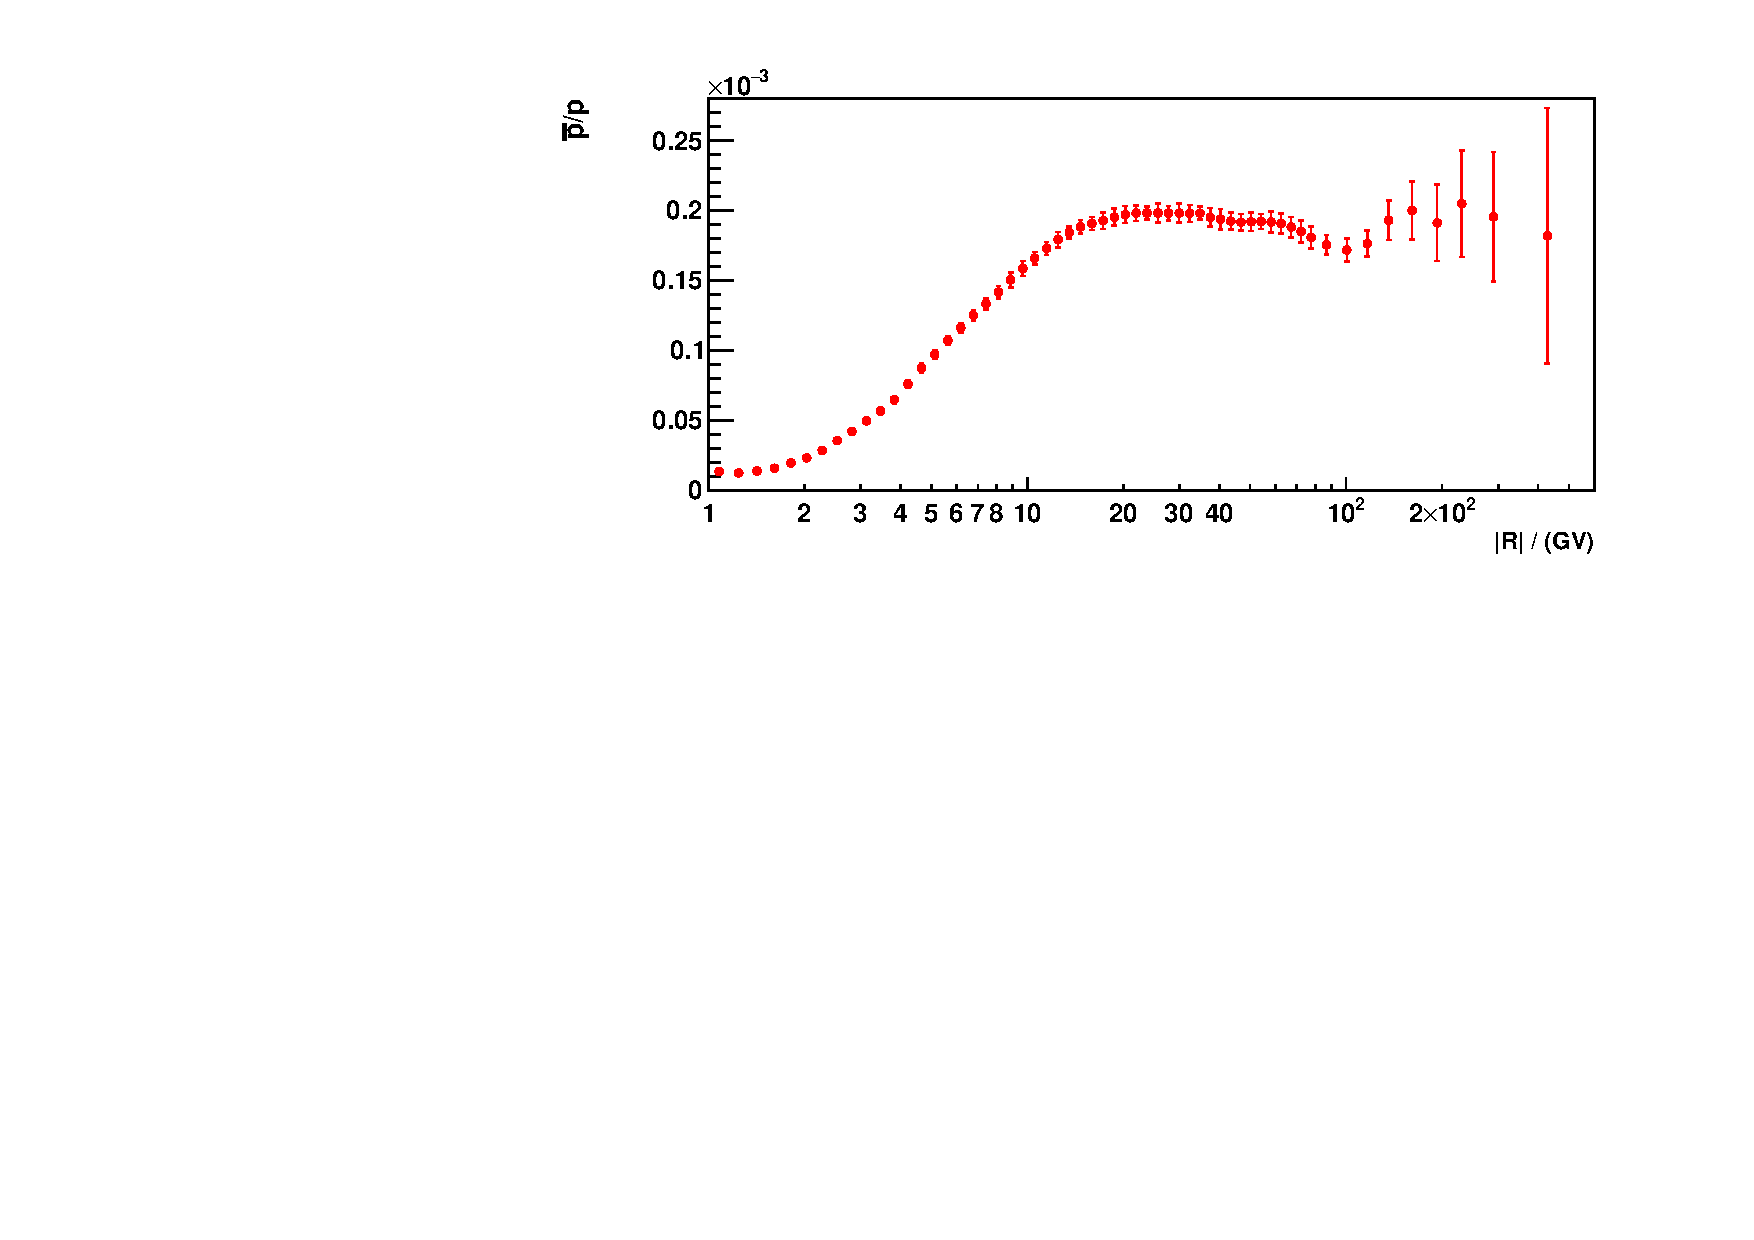
\includegraphics[width=1.0\textwidth, height=0.35\textheight]{Figures/chapter5/timeaveraged/fullratio_ThisAnallysisOnly_pass78.pdf} 
    \label{timeaveragedratio}
    }
    \subfigure[]{
	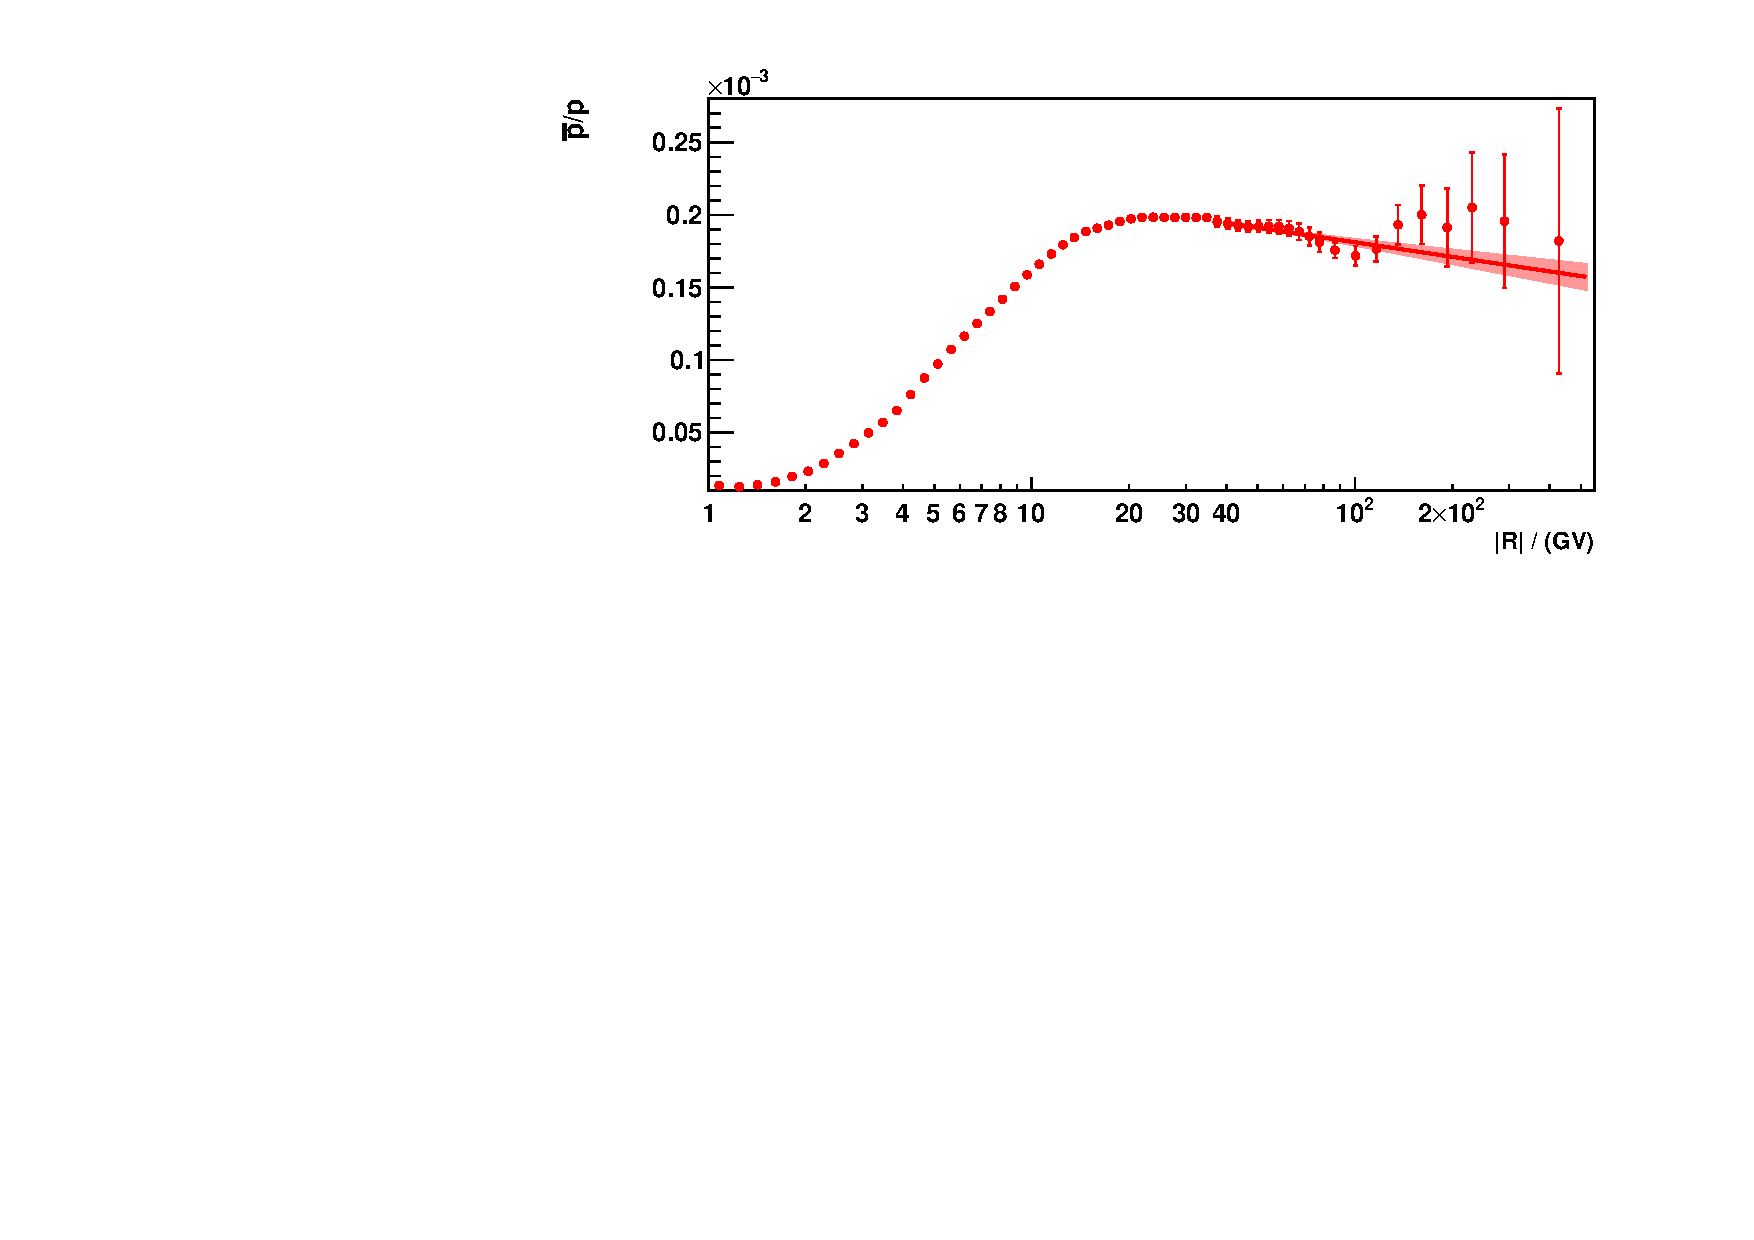
\includegraphics[width=1.0\textwidth, height=0.35\textheight]{Figures/chapter5/timeaveraged/Scaled_CorrelatedOnly/fullratio_ThisAnallysisOnly_pass78_LogXLinearY}
	\label{fullratio_ThisAnallysisOnly_LinearXLogY_WithFit}
    }
    \caption[The time-averaged antiproton to proton flux ratio.]{The time-averaged antiproton to proton flux ratio with the data collected from May 2011 to May 2021. a). Antiproton to proton flux ratio. The error bars are the total errors calculated from the quadratic sum of the statistical and the systematic errors; b). Linear fit above 40 GV on antiproton to proton flux ratio with statistical uncertainty and correlated systematic uncertainty only. The solid line shows the fit together with the 68\% C.L. ranges of the fit parameters (shaded regions).}    
\end{figure}



% Trend
%In figure \ref{fullratio_ThisAnallysisOnly_LinearXLogY_WithFit}, a linear fit in the antiproton to proton flux ratio is performed above 60.3 GV, this leads to a fitted slope $k$ = $(0.31\pm0.73)\times10^{-7}$ $\rm{GV}^{-1}$. Compared to the linear fit result in the same rigidity range in the previous AMS-02 publication \cite{AMS02AntiprotonPRL2016}, the observed behavior keeps the same. The antiproton to proton ratio is relatively flat in the high rigidity range. No obvious falling trend is observed as is the case for the positron to electron flux ratio shown in the latest paper by the AMS-02 collaboration \cite{PhysicsReport2}. In order to study the ratio in even higher rigidity ranges, more data is required and better charge confusion separation is needed. \par 
In figure \ref{fullratio_ThisAnallysisOnly_LinearXLogY_WithFit}, a linear fit in the antiproton to proton flux ratio with statistical uncertainty and correlated systematic uncertainty only is performed above 40 GV, this leads to a fitted slope $k$ = $(-1.44\pm0.42)\times10^{-5}$ $\rm{GV}^{-1}$. Compared to the result in the previous AMS-02 publication \cite{AMS02AntiprotonPRL2016}, the observed behavior keeps the same. The antiproton to proton ratio is relatively flat in the high rigidity range. No obvious falling trend is observed as is the case for the positron to electron flux ratio shown in the latest paper by the AMS-02 collaboration \cite{PhysicsReport2}. In order to study the ratio in even higher rigidity ranges, more data is required and better charge confusion separation is needed. \par 
%and a $\chi^2$/ndf=9.26/12=0.77


% Check with the publication
To check the consistency between the result of this analysis and the one published by the AMS-02 collaboration \cite{PhysicsReport2}, the antiproton to proton flux ratio is also determined in this analysis with the same data period, namely from May 2011 to Nov 2017. In figure \ref{PbarRatioCompareWithPhysicsReport}, the antiproton to proton flux ratio of this analysis based on six and a half years of data is shown in comparison with the AMS-02 published result in the Physics Report that is obtained for the same data period. The result of this analysis matches well the AMS-02 published result within the error bars except the first few points. Since the first three points significantly deviate, they are excluded in the time-dependent analysis. 

\begin{figure}[hptb]
\centering
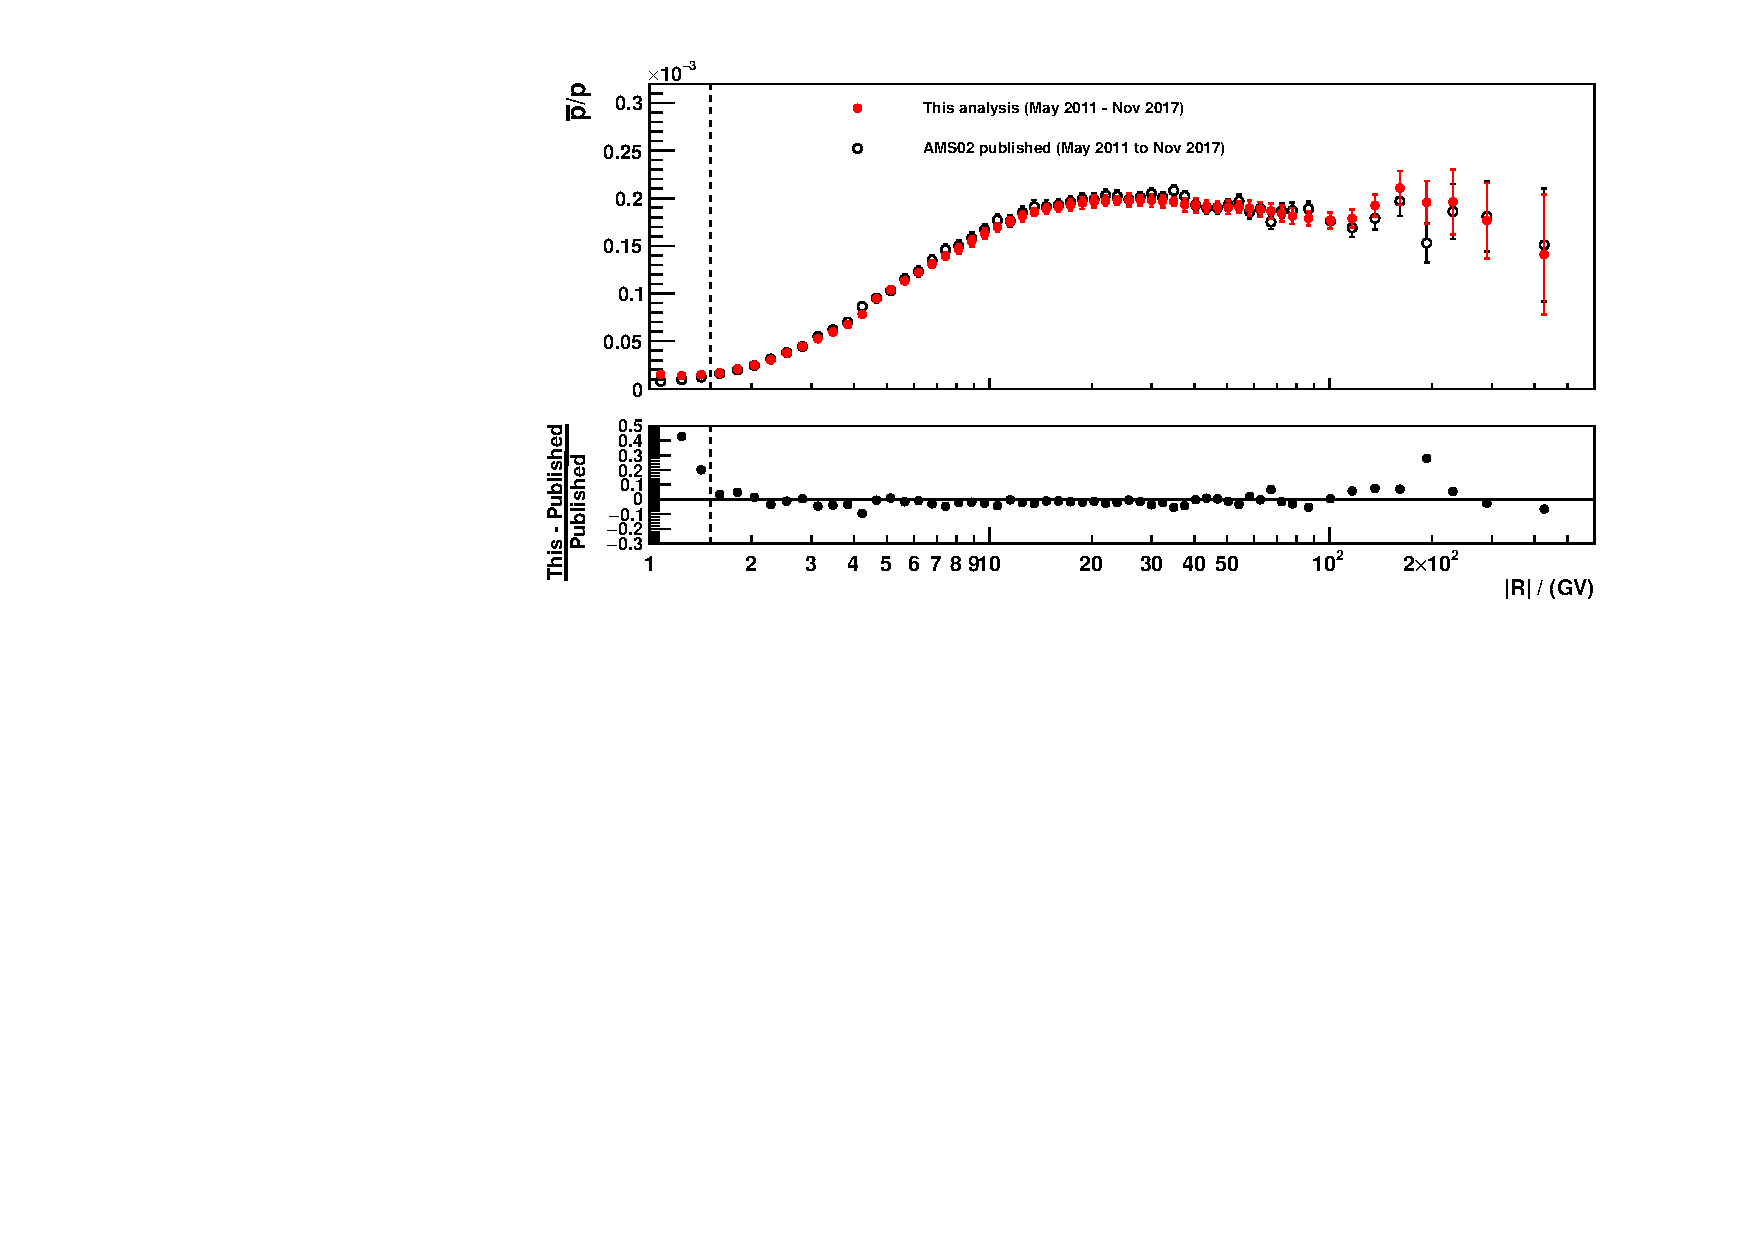
\includegraphics[width=1.0\textwidth, height=0.36\textheight]{Figures/chapter5/timeaveraged/fullratio_NOT_overlapped_PhysicsReport2021_PhyRep2021.pdf}
\caption[Comparison between the antiproton to proton flux ratio in this analysis and in the Physics Report.]{Comparison of the antiproton to proton flux ratio of this analysis to the AMS-02 published result in Physics Report \cite{PhysicsReport2}, for the same time interval of six and a half years. Both results agree well with each other within the error bars except the first few points. The statistic in the low rigidity range is highly subject to the geomagnetic cutoff as shown in figure \ref{IGRFvsStomer}. This could lead to a difference between the results. Therefore, the first three points (on the left of the dashed line) are excluded in the time-dependent analysis.}
\label{PbarRatioCompareWithPhysicsReport}
\end{figure}

% Time-averaged Pbar to Proton Ratio Error Breakdown
\begin{figure}[hptb]
\centering
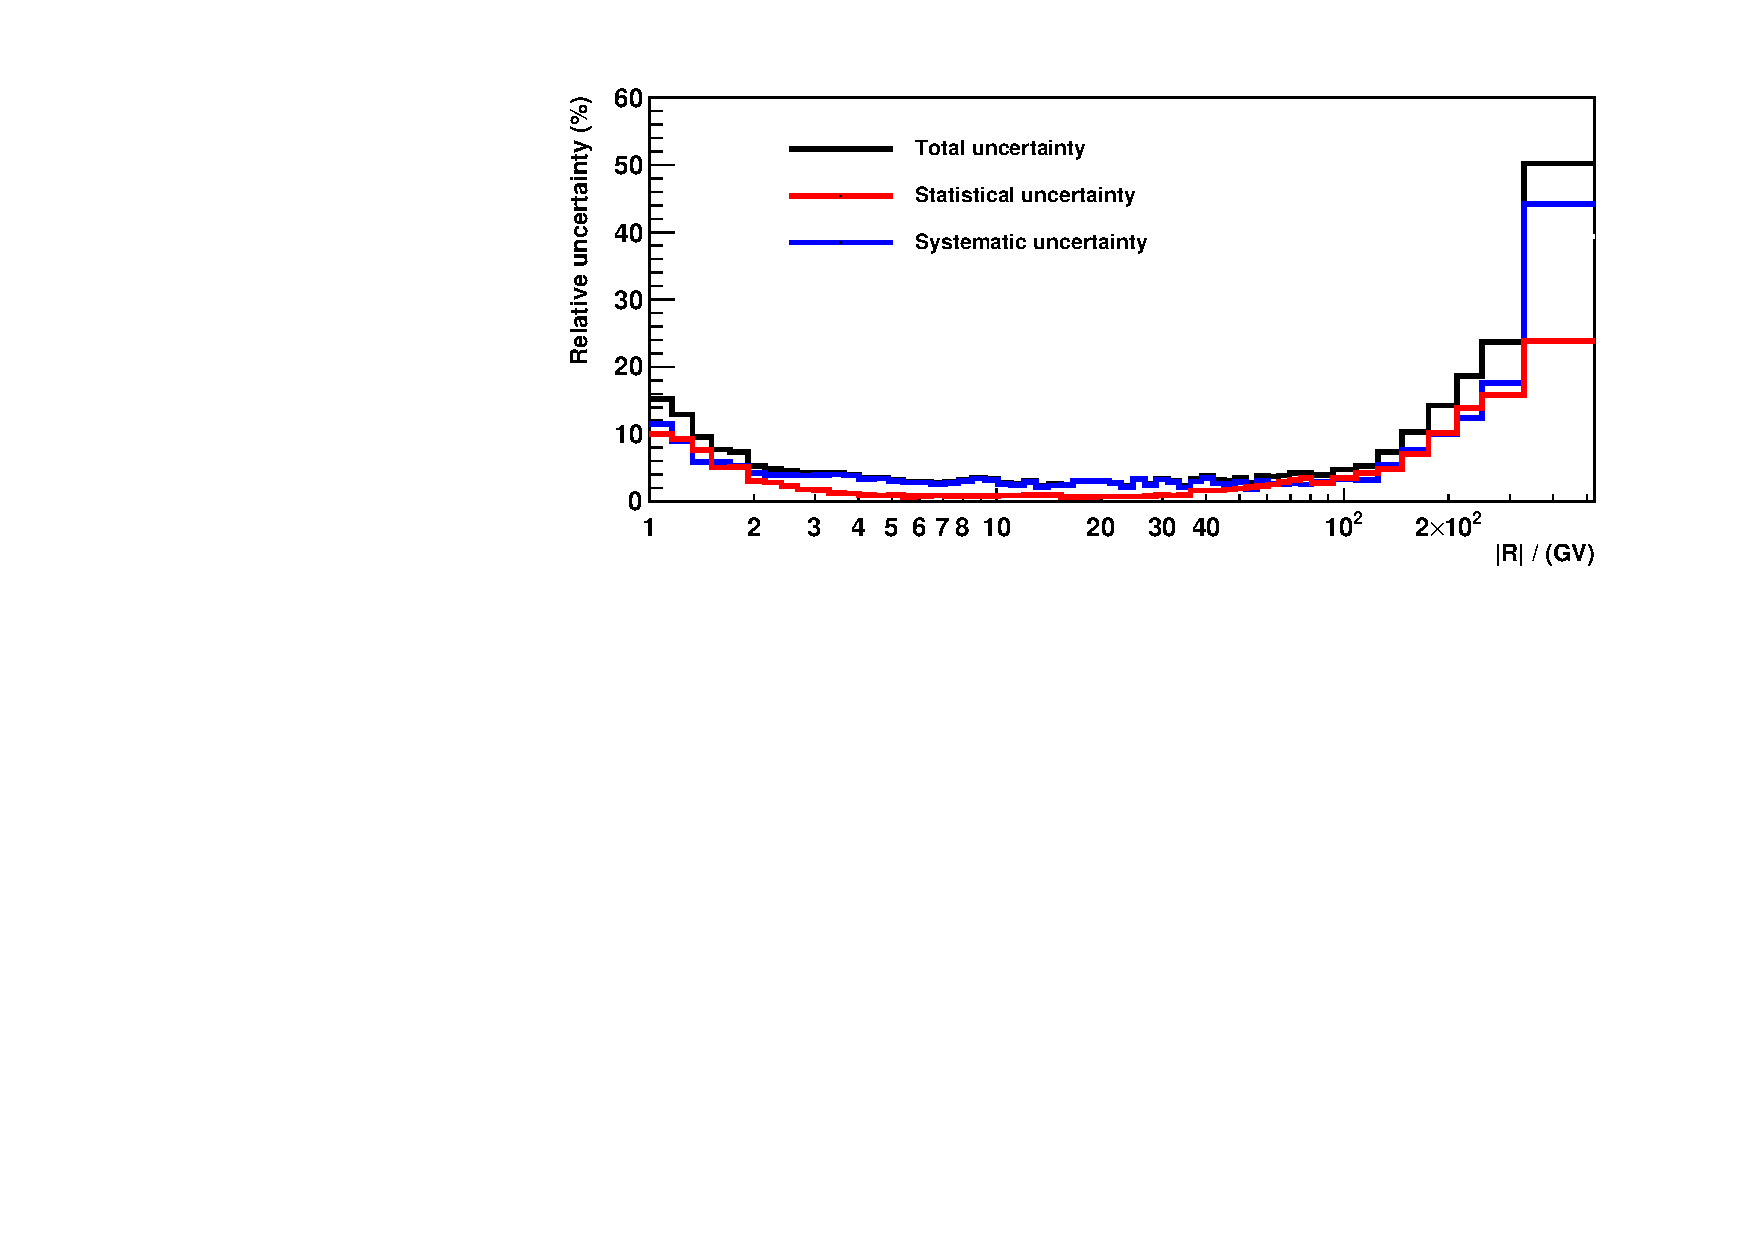
\includegraphics[width=1.0\textwidth, height=0.33\textheight]{Figures/chapter5/timeaveraged/TotalRelErr_BreakDown_pass78.pdf}
\caption[Uncertainty breakdown of the time-averaged antiproton to proton flux ratio.]{The uncertainty breakdown of the time-averaged antiproton to proton flux ratio in this analysis. In the highest rigidity bin, the systematic uncertainty is dominant due to the charge confused protons. In the low rigidity range, the statistical and systematic uncertainties are similar.}
\label{totalerrorbreakdown}
\end{figure}

The breakdown of the total uncertainty into its statistical and systematic components is shown in figure \ref{totalerrorbreakdown}. In the high rigidity range, the error is mainly dominated by the systematic error due to the background of charge confused protons and the limited separation power. In the intermediate rigidity range, the error is dominated by the systematic error due to the effective acceptance. In the low rigidity below 2 GV, the contributions from the statistical and the systematic uncertainties are at a similar level. \par
%which is an improvement when compared to the earlier AMS-02 result \cite{AMS02AntiprotonPRL2016, PhysicsReport2}. \par

In figure \ref{StaSysRelErrCompare}, the comparison of the total systematic and the statistical uncertainties between this analysis and the result in Physics Report \cite{PhysicsReport2} is shown. Although the analyzed data-taking period in this analysis is longer, the statistics do not gain significantly due to the frequent change of the TTCS and the cuts used in this analysis are stricter. Therefore the two independent results give statistical uncertainty at the same level. The systematic uncertainties of the two independent results match in the most rigidity range. But in the high rigidity range, due to the different $\Lambda_{\rm{CC}}$, the systematic uncertainties from the charge confusion, which is dominant in the high rigidity range, are different. \par


\begin{figure}[hptb]
\centering
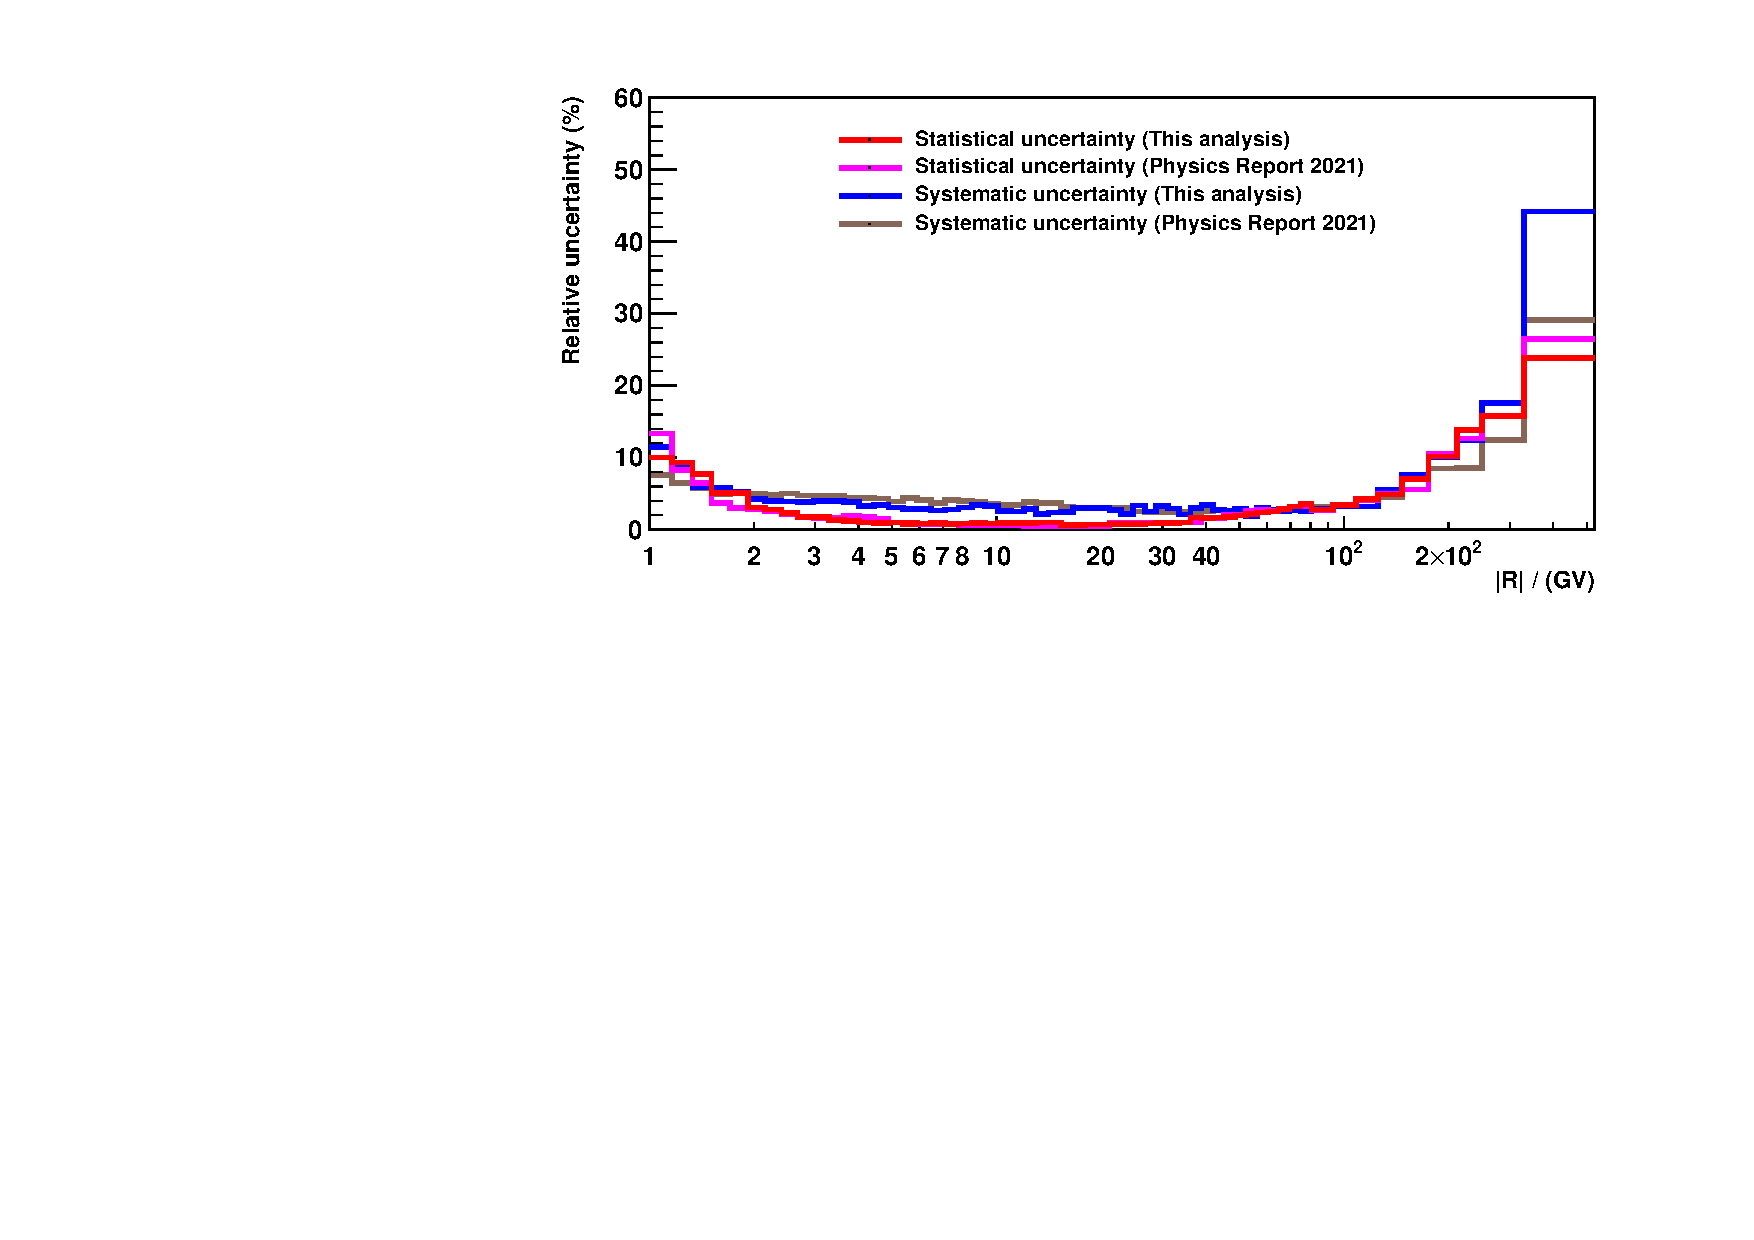
\includegraphics[width=1.0\textwidth, height=0.33\textheight]{Figures/chapter5/timeaveraged/StaSysRelErrCompare_pass78.pdf}
\caption[The statistical and systematic uncertainty comparison between this analysis and in Physics Report.]{The statistical and systematic uncertainty comparison between this analysis and AMS-02 publication in Physics Report \cite{PhysicsReport2}.}
\label{StaSysRelErrCompare}
\end{figure}
    
    
    
    
    